\documentclass[12pt,letterpaper,notitlepage]{article}

\usepackage{epsfig,amsmath,amssymb,cite,color,multirow,ulem,bm}

\usepackage{graphicx,wasysym}
\usepackage{hyperref}
\usepackage{tabulary}

\usepackage{pdfpages}
\usepackage{xcolor}

\usepackage{float}

\newcolumntype{K}[1]{>{\centering\arraybackslash}p{#1}}

\makeatletter
\newcommand{\thickhline}{%
    \noalign {\ifnum 0=`}\fi \hrule height 1pt
    \futurelet \reserved@a \@xhline
}
\newcolumntype{"}{@{\hskip\tabcolsep\vrule width 1pt\hskip\tabcolsep}}

\newcommand{\listintertext}{\@ifstar\listintertext@\listintertext@@}
\newcommand{\listintertext@}[1]{% \listintertext*{#1}
  \hspace*{-\@totalleftmargin}#1}
\newcommand{\listintertext@@}[1]{% \listintertext{#1}
  \hspace{-\leftmargin}#1}
\makeatother

\oddsidemargin 0cm
\evensidemargin 0cm
\marginparwidth 68pt
\marginparsep 10pt
\topmargin 0cm
\headheight 0pt
\headsep 0pt
\footskip 30pt
\textheight 22cm
\textwidth 16.5cm\textbf{}
\columnsep 10pt
\columnseprule 0pt

\newcommand{\tev}{\,\, \mathrm{TeV}}
\newcommand{\gev}{\,\, \mathrm{GeV}}
\newcommand{\mev}{\,\, \mathrm{MeV}}



\begin{document}

\begin{center}
\LARGE Scan over benchmarks
\end{center}

\vspace{1.0cm}
\begin{abstract}
\vspace{0.2cm}\noindent
The goal is to study more benchmarks and see, which directions in the parameter space would lead to the better signal-background discrimination.
\end{abstract}

\section{Exploring the parameter space}
The idea is to fix one of the parameters and to vary the rest in the following way (the graphical representation is swown on fig.\ref{fig:first-benchmarks}):
\begin{itemize}
  \item Keep $\Delta_m=m_C-m_l$ and $c \tau_C$ fixed (not changing the hardness of the leptons) and decrease $m_C$. This will increase the cross section and potentially $d_0$ (due to the slightly higher boost). Since we are in principle trying to explore the reach of our analysis to higher masses, we would suggest to first decrease the charged mass to 200 GeV, with a potential further decrease to 150 GeV.
  \item Keep $\Delta_m=m_C-m_l$ and $m_C$ fixed and increase  $c \tau_C$ (decrease the coupling r in code). This would show us, how much we win by making the displacement large. However, based on Table 4 from \cite{CMS:2016isf}, one can infer that the current $c \tau_C=2\ cm$ is probably the one with the highest sensitivity. In order to check this statement we propose to simulate events with $c \tau_C=10\ cm$ ($r=5e-9$ in code code).
  \item In order to check if we could reach for higher masses, we propose to have a look on the large mass splittings while fixing $c \tau_C$ and $m_C$. In principle, we could also slightly vary the PT-cut and look for similar effects. For now, we suggest to increase the mass splitting to $\Delta m=30$ GeV which would populate more the region above the current PT cut and hopefully make a better signal-background discrimination possible.
\end{itemize}

\begin{figure}[H]
\centering
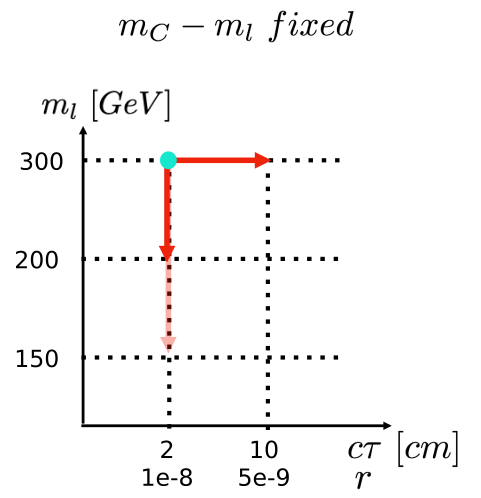
\includegraphics[height=2.5in]{fig-benchmarks/ctau-m.png}
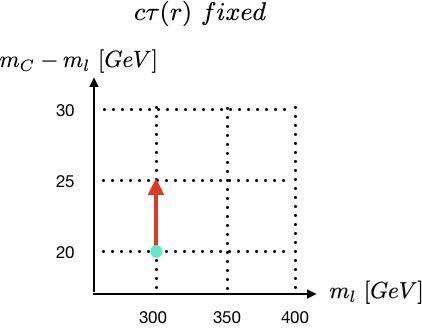
\includegraphics[height=2.5in]{fig-benchmarks/m-splitting.jpg}
\caption{\label{fig:first-benchmarks} Proposed directions in the parameter space. The current benchmark point is indicated by the cyan dot.}
\end{figure}
\newpage
\section{Finding an excluded point}
The task here is to find (at least one) point that we will be for sure able to exclude. An attractive idea to relate our model to the one considered in \cite{CMS:2016isf}, however, does not bring much of insight. The signal/background ratio in the search mentioned is much higher due to both higher production cross section and much larger pT. In the decays of the stops $\tilde{t_1}\rightarrow b l$ the transverse momentum of the lepton peaks around $pT=m_{\tilde{t_1}}/2$ which is of the order of $O(100)$ GeV. Thus, the higher-pT regions of the phase space a naturally more populated.

Nevertheless, the exclusion plot \ref{fig:CMS_exclusion} can still be used to find the point with the highest signal/background ratio in our model. In order to do so, let's find such model parameters $m_C,\ \Delta m,\ c\tau$ that would:
\begin{enumerate}
  \item Give the maximal signal cross section
  \item Will have the best sensitivity
\end{enumerate}
The first condition can be fulfilled by going to the small DM masses. The lightest mass not excluded by the LEP searches for any mass splitting is $m_l=100\ GeV$.

The sensitivity condition should have a peak in the $c\tau-\Delta m$ plane. Figure \ref{fig:CMS_exclusion} suggests that for the mass splittings of the order of $100\ GeV$ the sensitivity will peak at around $c \tau=2\ cm$.

This test should give us a rough understanding of how much to the left would the bound \ref{fig:CMS_exclusion} shift in our model (i.e. how much smaller masses could be excluded) due to the smaller cross section.

\textbf{To conclude, we suggest to test the parameter point $m_l = 100\ GeV, \Delta m=100\ GeV, c\tau=2\ cm$.}


\begin{figure}[H]
\centering
\includegraphics[height=3.2in]{fig-benchmarks/CMS_exclusion.png}
\caption{\label{fig:CMS_exclusion} Exclusion region from the displaced $e\mu$ search in \cite{CMS:2016isf}.}
\end{figure}

\begin{thebibliography}{6}

  \bibitem{CMS:2016isf}
    CMS Collaboration [CMS Collaboration],
    %``Search for displaced leptons in the e-mu channel,''
    CMS-PAS-EXO-16-022.


\end{thebibliography}

\end{document}
